\documentclass[10pt, tikz]{standalone}
\usetikzlibrary{arrows, math}

%	c3 = 1/100
%	c4 = -3/2000 
%	c5 = 3/50000

\begin{document}
	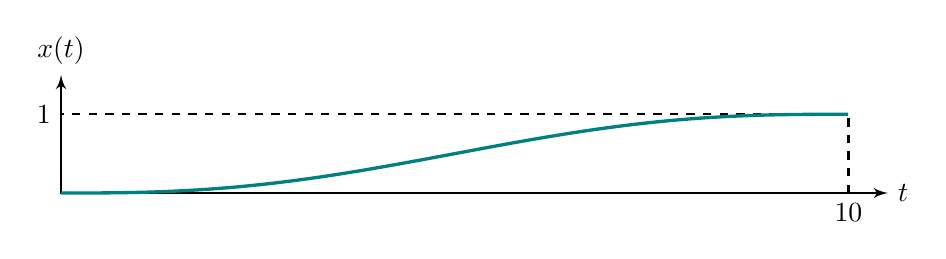
\begin{tikzpicture}[thick, scale=1]
		% eixos
		\draw [latex'-latex'] 
			(0, 1.5) node [above] {$x(t)$} -- (0,0) -- 
			(10.5, 0) node [right] {$t$}
		;
		\draw [dashed] 
			(10, 0) node [below] {$10$} -- (10, 1) -- 
			(0, 1) node [left] {$1$}
		;
		
		% x(t) = c3t^3 + c4t^4 + c5t^5
		\draw [very thick, teal] plot[variable=\t, domain=0:10, samples=250] 
			({\t}, {\t*(\t/10)*(\t/10) - 3*(\t/2)*(\t/10)*(\t/10)*(\t/10) + 3*(\t/5)*(\t/10)*(\t/10)*(\t/10)*(\t/10)})
		;
	\end{tikzpicture}
\end{document}